\chapter{Night 5}

\begin{learningobjectives}
\emph{Concepts}
\bi
\item Describe the physical significance of the mean and standard deviation of a data set.
\item Describe the physical significance of correlation, anti-correlation or non-correlation of two variables.
\item Approximate the mean and standard deviation from a histogram of the data.
\item Interpret the meaning of a pair of images that has a Pearson Correlation Coefficient of:  about 0; or 0.5; or 0.9. 
\item Interpret the physical/mathematical meaning of the diagonal and off-diagonal elements in a 2 x 2 correlation matrix, $\mathbf{C} = \mathbf{A}^T\mathbf{A}$, if given the equation for the Pearson Correlation Coefficient. 

\ei
\emph{MATLAB skills}
\bi
\item Compute the dot product of two vectors
\item Set up the appropriate matrices to compute the correlation coefficient between two variables.
\ei
\end{learningobjectives}

\section{Correlation}

Now let's consider that we measure two different associated quantities and want to test whether these are linearly correlated (if one goes up, the other also goes up), anti-correlated (if one goes up the other goes down) or uncorrelated (the behavior of one cannot be predicted by watching the behavior of the other).  (Please note that correlation has nothing to do with causality!).  There are many different measures of correlation, but we will discuss here one of the most common, the Pearson Correlation Coefficient.

For a pair of associated datasets $X = \{x_i\}$ and $Y = \{y_i\}$, each with $n$ elements, we define the Pearson Correlation Coefficient to be:
\begin{equation}
\rho(X,Y) = \frac{\sum_{i=1}^n (x_i - \mu_x)(y_i - \mu_y)}{(N-1) \sigma_x \sigma_y}
\end{equation}
where $\mu_x$, $\mu_y$, $\sigma_x$ and $\sigma_y$ are the means and standard deviations of the datasets.  Essentially, for each pair of values, we take the product of the variations from the mean, then sum these products up over all pairs of values and normalize by the expected variation as characterized by the standard deviation.  If the two values are consistently always on the same side of the mean, then each term in the sum will contribute positively, and the total value will be close to one, indicating positive correlation.  If the two values are consistently on the opposite sides of the mean, then each term in the sum will contribute negatives, and the total value will be close to negative one, indicating anticorrelation.  If, for every pair, it is just as likely that the two values will be on opposite sides of the mean as on the same side of the mean, then the sum will go to zero, and the two values are uncorrelated.


Consider the following data:

\begin{center}
  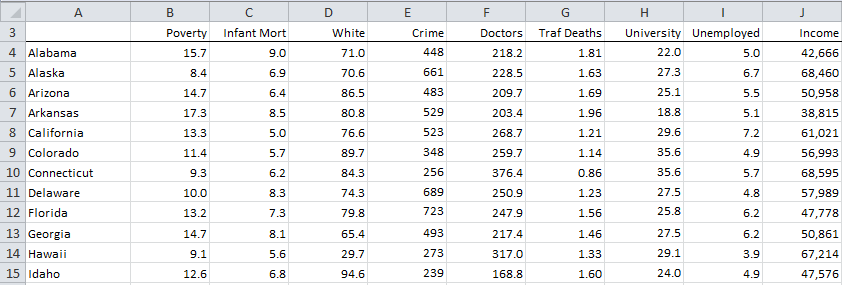
\includegraphics[width=4in]{FacesNight3/figs/us-states-statistics.png}
\end{center}

\begin{prob}
\begin{enumerate}
\item Look over the data.  By eye, which columns look correlated?  Anticorrelated? Uncorrelated?
\item  Choose your two favorite columns of data from this dataset.  Input these into vectors in Matlab.  For each of these vectors, subtract off the mean, and then divide out the standard deviation.
\item With these vectors, how would you directly compute the correlation coefficient between them? Go ahead and do this in MATLAB, and reflect on your result.
\end{enumerate}
\end{prob}

A note of warning.  Correlation does not imply causation.
\begin{prob}
To drive this point home, visit the \href{http://tylervigen.com/spurious-correlations}{Spurious Correlation Website}.  Follow the link at the bottom of the site to discover and plot a spurious correlation of your very own.
\end{prob}

\section{Correlation: The Idea, the Math, and the MATLAB}
Here we are going to consider a matrix like the one you constructed above, based on the datasets, which has elements of the correlation coefficients.  Let's first consider a matrix $\mathbf{B}$ which has the datasets as columns:
\begin{align*}
\mathbf{B} =  \begin{pmatrix}
    x_1 & y_1\\
    x_2 & y_2 \\
    x_3 & y_3\\
    ...&...\\
  \end{pmatrix}
\end{align*}
If we subtract out the means and divide out the standard deviation and a factor of square root of $N-1$, we get the matrix $\mathbf{A}$:
\begin{align*}
\mathbf{A} = \frac{1}{\sqrt{N-1}} \begin{pmatrix}
    \frac{x_1-\mu_x}{\sigma_x} & \frac{y_1-\mu_y}{\sigma_y}\\
   \frac{x_2-\mu_x}{\sigma_x} &  \frac{y_2-\mu_y}{\sigma_y}\\
    \frac{x_3-\mu_x}{\sigma_x} & \frac{y_3-\mu_y}{\sigma_y}\\
    ...&...\\
  \end{pmatrix}
\end{align*}
where $\mu_x,\mu_y$ and $\sigma_x,\sigma_y$  are the mean  and standard deviations of each column, and $N$ is the number of samples (rows).  Now we
can write the \textit{correlation matrix} as $\mathbf{C} = \mathbf{A}^T \mathbf{A}$ which has elements of the self and cross correlations between the datasets.

\begin{prob}\label{ex:matlab-cor}
\begin{enumerate}
\item Before we start to use this idea, let's think through it a bit...
\begin{enumerate}
    \item  What is the size of the matrix $\mathbf{C}$?
    \item What are the elements on the \textit{diagonal} of this matrix?
    \item What are the elements of the off-diagonal?  What is element $C_{12}$ of this matrix?  What is element $C_{21}$?  What do you notice?  Is this always going to be true?  What about if we had three datasets?  What can you say about the elements $C_{13}$ vs $C_{31}$?
    \item  If you create a data matrix that has completely identical columns of data, what should the correlation matrix look like?
    \item  If you create a data matrix that has completely uncorrelated datasets, what should the correlation matrix look like?
\end{enumerate}
\item Now let's actually implement this. For the sake of getting you more comfortable manipulating matrices in MATLAB, do the following at the command line, and see if you can predict what each term will do before you type it in.  For each command, explain what MATLAB is doing.

\begin{verbatim}
>> a = [(1:10)',rand(10,1)]
>> o = ones(size(a,1),1)
>> m = o*mean(a)
>> s = o*std(a)
>> b = (a-m)./s
>> c=(1/(size(a,1)-1))*b'*b
\end{verbatim}
\item What would happen if you used this matrix for a instead:
\begin{verbatim}
>> a = [(1:10)',(1:10)'/2 -(1:10)' ]
\end{verbatim}
Make a prediction, and try it out.
\item Now learn how to use the MATLAB function \texttt{corrcoef}, which will compute the correlation coefficients using the original matrix.
%\item  Now that you've got a handle on doing this in MATLAB, test your correlation-finding abilities with a real application.  Online, there are many many publicly available datasets.  In particular, the listing at \begin{verbatim} http://www.stat.ufl.edu/~winner/datasets.html \end{verbatim}  has a great set of data suitable for correlation testing. (Look at the linear regression datasets about a fifth of the way down the page).  Pick one to test for correlation.  What will you find?  Does LSD consumption correlate with improved math test scores?  In hybrid vehicles, which correlated more strongly with price:  mileage or acceleration?  Explore!  (Please note however, we are scratching the surface of data science here.  There is a lot more to learn, and not every dataset on this page will be suitable for linear correlation analysis).
\end{enumerate}
\end{prob}
\begin{sol}
\begin{enumerate}
    \item \begin{enumerate}
        \item Since $\mathbf{A}$ has size $N \times 2$, we know $\mathbf{A}^T$ has size $2 \times N$. Then $\mathbf{C} = \mathbf{A}^T\mathbf{A}$ has size $2 \times 2$.
        \item Each element of the diagonal will be 1.
        \item The elements $\mathbf{C}_{12}=\mathbf{C}_{21}$ is the correlation between the two columns of data. Regardless of size, the correlation matrix will be symmetric.
        \item If the data matrix had identical columns of data, the correction matrix would be all 1s.
        \item If the data is uncorrelated, the off-diagonal entries in the correlation matrix will be all 0s, so it will be the identity matrix. (Note: real data is unlikely to have 0 correlation, just by accident, so it will just have numbers that are close to 0.)
    \end{enumerate}
    \item You should end up with a correlation matrix between the two columns of \texttt{a}.
    \item Again, you end up with a correlation matrix between the two columns of \texttt{a}, but since the numbers are non-random and negatively correlated, you get the matrix $\mathbf{c}=\begin{bmatrix} 1 & -1 \\ -1 & 1\end{bmatrix}$.
    \item You should use ``help'' or ``doc'' to find information on how to use this function.
\end{enumerate}
\end{sol}

\section{From Data to Dimensions}

Thus far we've made a distinction between vectors as representing points in space, and vectors as representing data (e.g., a list of intensity values for pixels).  But if you wanted to, there's no reason you couldn't think of a vector of $n$ data points as representing a point in $n$ dimensional space (and, in fact, it would be very powerful \textit{to}).  If you did this, you could define all kinds of interesting things. For example, you could ask about the magnitude of the vector (i.e., the size of a data point), the distance from one vector (i.e., data point) to another, the dot product of two vectors (i.e., data points), etc.

\begin{prob}
\begin{enumerate}
\item As a thought experiment, think about the following questions.
\begin{enumerate}
\item Imagine you have grayscale images that are $100 \times 100$ pixels.  If you represent each image as a vector, how large is the vector space?
\item If the intensity of pixel $ij$ is $a_{ij}$, come up with an expression for the magnitude of the vector that describes the image $\mathbf{a}$.
\item Come up with an expression that represents the distance between images $\mathbf{a}$ and $\mathbf{b}$.
\item What does $\mathbf{a}^T\mathbf{b}$ tell you?  What vector operation is this?

    \end{enumerate}
\item Now that you've thought through this about, load three face images, and calculate the distance between each pair (i.e., take the difference between the two images, square each element, then sum up all the squared elements and take the square root of the sum).  Do your answers make sense?
\end{enumerate}
\end{prob}
\begin{sol}
\begin{enumerate}
    \item Each pixel is represented by a number. So the vector representing an image has $10000$ entries and thus lives in $10000$-dimensional space.
    \item The magnitude of the vector is given by
    $$\|\mathbf{a}\| = \left(\sum_{i,j} a_{i,j}^2\right)^{1/2}.$$
    \item The distance between two images $\mathbf{a}$ and $\mathbf{b}$ is given by
    $$\|\mathbf{a}-\mathbf{b}\| = \left(\sum_{i,j} (a_{i,j}-b_{i,j})^2\right)^{1/2}.$$
    \item The dot product $\mathbf{a}^T\mathbf{b}$ tells you how similar the two vectors are.
\end{enumerate}
\end{sol}

\section{Correlation in Facial Recognition}

\subsection{Kinds of Correlation in an Image Set}

If we think about pictures now, we can think about two different correlations:  the correlation between a given pair of pixels (across all the pictures in a data set), and the correlation between pictures (across all the pixels in those images). In order to compute an accurate correlation coefficient, you need to have multiple data points in each set being correlated, e.g., many pixels in each picture being correlated, or many pictures across which a pair of pixels (pixel locations) can be correlated.

Think about what each of these correlations \textit{means}.  What would a high correlation between a given pair of images mean?  What about a high correlation between a given pair of pixels (e.g., the upper-left-most pixel and the upper-right-most pixel)? It might help to open a few face images or draw some face sketches to think about.

\begin{prob}
Consider six grayscale pictures, each with a resolution of $m$ x $n$ pixels.
    \begin{enumerate}
    \item  What is the size of the data matrix containing these six pictures as the columns?

    \item  What is the expression for the correlation matrix between the pictures?  What size is this correlation matrix?

    \item  What is the expression for the correlation matrix between different pixels? Pay careful attention to the mean and standard deviation you are using.  What is the size of this correlation matrix?
    \item People's faces are approximately left-right symmetric.  How would you expect this to affect the entries in the correlation matrix between different pixels?
\end{enumerate}
\end{prob}
\begin{sol}
\begin{enumerate}
    \item Each picture is represented by $mn$ data points. So the data matrix containing these six pictures as columns is $mn \times 6$.
    \item To find the correlation we can either use the MATLAB code from Exercise~\ref{ex:matlab-cor} or the command \texttt{corrcoef}. The correlation matrix will be $6 \times 6$.
    \item To find the correlation between pixels, we need to take the transpose of our data matrix. This new data matrix will be $6 \times mn$, since we have $mn$ variables (each pixel) and 6 observations (within in picture). The correlation matrix will then be $mn \times mn$.
    \item High correlation between pixels equidistant from centerline.
\end{enumerate}
\end{sol}

\subsection{Test your understanding...}
\begin{itemize}
\item  Pull in \textbf{six images} from the class data matrix (\texttt{test\_images} variable in \texttt{face\_bases.mat} file) and put them in a variable called \texttt{faces}.
Each of these images should come from different people - there are 8 images per person stored in the data matrix.
\item Use the \texttt{resample} command to bring them down to a smaller resolution (e.g., 25 x 25) using\\
\texttt{dfaces = imresize(faces,[25 25]);}\\
his should be a 25 x 25 x 6 matrix.
\item Now reshape them appropriately to create a matrix in which each column is a (reshaped) face using\\
\texttt{rdfaces =  reshape(dfaces,size(dfaces,1) * size(dfaces,2),size(dfaces,3));}\\
\end{itemize}

\begin{prob}
\begin{enumerate}
\item Find the correlation between six different images.  Which images have the highest correlation?
\item Now find the correlation between pixels across images. Try taking a single column of this matrix and reshape that column into an image.  What does that image tell you? You may want to repeat this reshape and visualization for columns 1, 25, 400, and 625 to get a feel for what is happening.
\end{enumerate}
\end{prob}
\begin{sol}
\begin{enumerate}
    \item To find the correlation matrix between the six images, enter\\ \texttt{>> corrcoef(rdfaces)}. 
    \item To find the correlation across pixels, enter\\ \texttt{>> pixels=corrcoef(transpose(rdfaces));}. We can reshape the first column of this matrix and convert it into an image using\\
    \texttt{>> pixels1=reshape(pixels(:,1),25,25);}\\
    \texttt{>> imagesc(pixels1).}\\
    The $(i,j)$ entry of this image tells us how similar the top-left pixel is to the $(i,j)$ pixel. (Note: the pixels are ``numbered'' 1--625 going down the first column, then down the second column, and so on.) Repeating this reshape and visualization procedure on column 400 will give you the correlation between pixel 400 and each of the other pixels, for example.
\end{enumerate}
\end{sol}

\section{Diagnostic Quiz}

Please see Canvas for the questions.

\pagebreak
\shipoutAnswer
